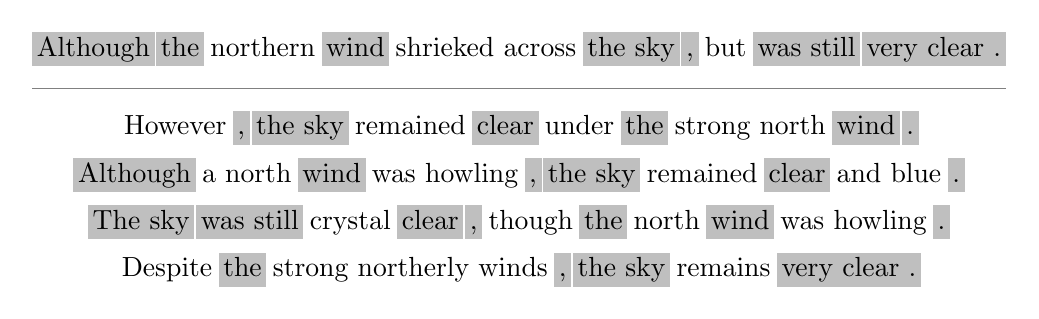
\begin{tikzpicture}[node distance=0.6cm]
	\tikzstyle{eval hilite}=[fill=lightgray]

	% hypothesis
	\matrix (sentence) [inner sep=0pt,column sep=1pt,nodes={inner sep=1.5pt,anchor=mid}]{
		\node (segment 0) {Although}; &
		\node (segment 1) {the}; &
		\node (segment 2) {northern}; &
		\node (segment 3) {wind}; &
		\node (segment 4) {shrieked across}; &
		\node (segment 5) {the sky}; &
		\node (segment 6) {,}; &
		\node (segment 7) {but}; &
		\node (segment 8) {was still}; &
		\node (segment 9) {very clear .}; \\
	};
	\path[eval hilite] 
		(segment 0.north west |- sentence.north west) rectangle (segment 0.south east |- sentence.south west);
	\path[eval hilite] 
		(segment 1.north west |- sentence.north west) rectangle (segment 1.south east |- sentence.south west);
	\path[eval hilite] 
		(segment 3.north west |- sentence.north west) rectangle (segment 3.south east |- sentence.south west);
	\path[eval hilite] 
		(segment 5.north west |- sentence.north west) rectangle (segment 5.south east |- sentence.south west);
	\path[eval hilite] 
		(segment 6.north west |- sentence.north west) rectangle (segment 6.south east |- sentence.south west);
	\path[eval hilite] 
		(segment 8.north west |- sentence.north west) rectangle (segment 8.south east |- sentence.south west);
	\path[eval hilite] 
		(segment 9.north west |- sentence.north west) rectangle (segment 9.south east |- sentence.south west);
	
	\node at (segment 0) {Although};
	\node at (segment 1) {the};
	\node at (segment 3) {wind};
	\node at (segment 5) {the sky};
	\node at (segment 6) {,};
	\node at (segment 8) {was still};
	\node at (segment 9) {very clear .};

	\path (sentence.west) -- +(0cm,-0.5cm) coordinate (separator start);
	\draw[thin,gray] (separator start) -- (separator start -| sentence.south east);

	% first reference sentence 
	\matrix (sentence) [inner sep=0pt,column sep=1pt,nodes={inner sep=1.5pt,anchor=mid},below of=sentence,node distance=1cm]{
		\node (segment 0) {However}; &
		\node (segment 1) {,}; &
		\node (segment 2) {the sky}; &
		\node (segment 3) {remained}; &
		\node (segment 4) {clear}; &
		\node (segment 5) {under}; &
		\node (segment 6) {the}; &
		\node (segment 7) {strong north}; &
		\node (segment 8) {wind}; &
		\node (segment 9) {.}; \\
	};
	\path[eval hilite] 
		(segment 1.north west |- sentence.north west) rectangle (segment 1.south east |- sentence.south west);
	\path[eval hilite] 
		(segment 2.north west |- sentence.north west) rectangle (segment 2.south east |- sentence.south west);
	\path[eval hilite] 
		(segment 4.north west |- sentence.north west) rectangle (segment 4.south east |- sentence.south west);
	\path[eval hilite] 
		(segment 6.north west |- sentence.north west) rectangle (segment 6.south east |- sentence.south west);
	\path[eval hilite] 
		(segment 8.north west |- sentence.north west) rectangle (segment 8.south east |- sentence.south west);
	\path[eval hilite] 
		(segment 9.north west |- sentence.north west) rectangle (segment 9.south east |- sentence.south west);
	\node at (segment 1) {,};
	\node at (segment 2) {the sky};
	\node at (segment 4) {clear};
	\node at (segment 6) {the};
	\node at (segment 8) {wind};
	\node at (segment 9) {.};

	% second reference sentence
	\matrix (sentence) [inner sep=0pt,column sep=1pt,nodes={inner sep=1.5pt,anchor=mid},below of=sentence]{
		\node (segment 0) {Although}; &
		\node (segment 1) {a north}; &
		\node (segment 2) {wind}; &
		\node (segment 3) {was howling}; &
		\node (segment 3 2) {,}; & % oops
		\node (segment 4) {the sky}; &
		\node (segment 5) {remained}; &
		\node (segment 6) {clear}; &
		\node (segment 7) {and blue}; &
		\node (segment 8) {.}; \\
	};
	\path[eval hilite] 
		(segment 0.north west |- sentence.north west) rectangle (segment 0.south east |- sentence.south west);
	\path[eval hilite] 
		(segment 2.north west |- sentence.north west) rectangle (segment 2.south east |- sentence.south west);
	\path[eval hilite] 
		(segment 4.north west |- sentence.north west) rectangle (segment 4.south east |- sentence.south west);
	\path[eval hilite] 
		(segment 6.north west |- sentence.north west) rectangle (segment 6.south east |- sentence.south west);
	\path[eval hilite] 
		(segment 8.north west |- sentence.north west) rectangle (segment 8.south east |- sentence.south west);
	\path[eval hilite] 
		(segment 3 2.north west |- sentence.north west) rectangle (segment 3 2.south east |- sentence.south west);
	\node at (segment 0) {Although};
	\node at (segment 2) {wind};
	\node at (segment 3 2) {,};
	\node at (segment 4) {the sky};
	\node at (segment 6) {clear};
	\node at (segment 8) {.};

	% third reference sentence
	\matrix (sentence) [inner sep=0pt,column sep=1pt,nodes={inner sep=1.5pt,anchor=mid},below of=sentence]{
		\node (segment 0) {The sky}; &
		\node (segment 1) {was still}; &
		\node (segment 2) {crystal}; &
		\node (segment 3) {clear}; &
		\node (segment 4) {,}; &
		\node (segment 5) {though}; &
		\node (segment 6) {the}; &
		\node (segment 7) {north}; &
		\node (segment 8) {wind}; &
		\node (segment 9) {was howling}; &
		\node (segment 10){.};\\
	};
	\path[eval hilite] 
		(segment 0.north west |- sentence.north west) rectangle (segment 0.south east |- sentence.south west);
	\path[eval hilite] 
		(segment 1.north west |- sentence.north west) rectangle (segment 1.south east |- sentence.south west);
	\path[eval hilite] 
		(segment 3.north west |- sentence.north west) rectangle (segment 3.south east |- sentence.south west);
	\path[eval hilite] 
		(segment 4.north west |- sentence.north west) rectangle (segment 4.south east |- sentence.south west);
	\path[eval hilite] 
		(segment 6.north west |- sentence.north west) rectangle (segment 6.south east |- sentence.south west);
	\path[eval hilite] 
		(segment 8.north west |- sentence.north west) rectangle (segment 8.south east |- sentence.south west);
	\path[eval hilite] 
		(segment 10.north west |- sentence.north west) rectangle (segment 10.south east |- sentence.south west);
	\node at (segment 0) {The sky};
	\node at (segment 1) {was still};
	\node at (segment 3) {clear};
	\node at (segment 4) {,};
	\node at (segment 6) {the};
	\node at (segment 8) {wind};
	\node at (segment 10) {.};

	% fourth reference sentence
	\matrix (sentence) [inner sep=0pt,column sep=1pt,nodes={inner sep=1.5pt,anchor=mid},below of=sentence]{
		\node (segment 0) {Despite}; &
		\node (segment 1) {the}; &
		\node (segment 2) {strong northerly winds}; &
		\node (segment 3) {,}; &
		\node (segment 4) {the sky}; &
		\node (segment 5) {remains}; &
		\node (segment 6) {very clear .}; \\
	};
	\path[eval hilite] 
		(segment 1.north west |- sentence.north west) rectangle (segment 1.south east |- sentence.south west);
	\path[eval hilite] 
		(segment 3.north west |- sentence.north west) rectangle (segment 3.south east |- sentence.south west);
	\path[eval hilite] 
		(segment 4.north west |- sentence.north west) rectangle (segment 4.south east |- sentence.south west);
	\path[eval hilite] 
		(segment 6.north west |- sentence.north west) rectangle (segment 6.south east |- sentence.south west);
	\node at (segment 1) {the};
	\node at (segment 3) {,};
	\node at (segment 4) {the sky};
	\node at (segment 6) {very clear .};



\end{tikzpicture}